\chapter{Megvalósítás}
\section{A szoftver feladatai}
A konkrét implementáció a BME IIT robotlaborjában történt egy Mitsubishi robotkaron. A komplett, több komponensből álló szoftver feladatai a következők:

\begin{itemize}
\item A robotkar mozgatása a PC-n bevitt helyzetbe.
\item A kéz-szem kalibráció automatikus elvégzése.
\item A 3D rekonstrukció elvégzése.
\item A tárgy helyzetének meghatározása 3D pontfelhőt tartalmazó adatbázis alapján.
\end{itemize}	

\section{Kiválasztott implementáció}
A tárgy helyzetének meghatározásához készítünk egy képet a tárgyról. Ezen a képen kulcspontkeresést hajtunk végre, majd párosítjuk ezeket a pontokat a 3D pontfelhő pontjaival. A pozíció és orientáció becslése PnP algoritmussal történik.

Az előző fejezetekben a legtöbb probléma megoldására több módszert is ismertettem. Itt szeretném bemutatni az implementációhoz kiválasztottakat.

\subsection{Kulcspontkeresés és -párosítás implementációja}
A kulcspontkeresés SURF algoritmussal történik. 

A párosító algoritmus minden esetben a \ref{matching} szakaszban ismertetett brute force párosító, mivel az több párosítást eredményez, mint a FLANN algoritmus. 

A 3D rekonstrukció során a kulcspontpárosításnál ismerjük a külső paramétereket, ezért a \ref{match-epilines} és \ref{match-homogr} szakaszokban ismertetett, epipoláris egyeneseket és homográfiát használó szűrést alkalmazom. A homográfiás szűrés esetén RANSAC elvű algoritmust használok.

Mivel a tárgy pozíciójának becslésekor épp a külső paramétereket kívánjuk meghatározni, ezért itt az epipoláris egyenesek használata nem lehetséges. Ennél a lépésnél a \ref{match-cross} szakaszban ismertetett keresztellenőrzéses szűrést alkalmazom.

\subsection{A kéz-szem kalibráció implementációja}

A kéz-szem kalibrációnál különböző nézőpontokból képeket kell készíteni egy kalibráló objektumról. Először az orientáció megtartásával, majd annak változtatásával. Sajnos a megvalósításhoz használt robotkar munkatere nem túl nagy, valamint a kamera látószöge is elég kicsi, ezért a kamera helyzetét nem lehet széles tartományban változtatni. Ez a kéz-szem kalibráció esetében az első fázisban (állandó orientáció) $\pm 5$ cm-es tartományt jelent mindhárom tengely mentén. Így a program 11 képet készít mind az $x$, $y$ és $z$ tengely mentén. A második fázisban a kalibráló objektum közepét a kép közepén tartva különböző szögekből készít képeket az algoritmus. Az $x$ tengely körül $\pm 15°$ elfordulást képes megvalósítani, az $y$ tengely körül a $\left[-9°, +30°\right]$ tartományban lehet változtatni az orientációt. Mindkét irányban szintén 11-11 képet készít a program.

A kalibráló objektum egy sakktáblamintázat volt, amit a \ref{fig:reconstr-img} ábrán is láthatunk. A minta sarokpontjainak meghatározásához az OpenCV-ben kész függvény van megírva, ezért ez nagyban megkönnyíti a kalibráció implementálását.

\subsection{3D rekonstrukció és a kéz-szem kalibráció implementációja}

A 3D rekonstrukció során a megtalált kulcspontpárok alapján a program egyszerű háromszögeléssel számít 3D pozíciót. A többnézetes háromszögelés módszerét végül elvetettem. 

Ahogy a kéz-szem kalibrációnál, úgy a 3D rekonstrukciónál is különböző nézőpontból kell képeket készíteni. Itt azonban a rekonstruálandó tárgyról készülnek a képek. Itt is probléma a limitált munkatér. A megvalósítás során az egyik tengely mentén $\left[-10°, +30°\right]$, a másik mentén pedig $\pm 30°$ tartományban készít a program képeket a tárgyról. A képek középpontjában ugyanúgy a tárgy "középpontját" tartja, viszont a két tengely körüli elforgatást egymástól függetlenül hajtja végre. Mindkét irányban 7 pontra osztottam fel az elfordulást, így összesen 49 kép készül a tárgyról. A külső paraméterek meghatározásához PnP algoritmust használ a program. Ugyanazt a sakktáblamintát használom, mint a kalibráció során.

\begin{figure}[H]
\centering
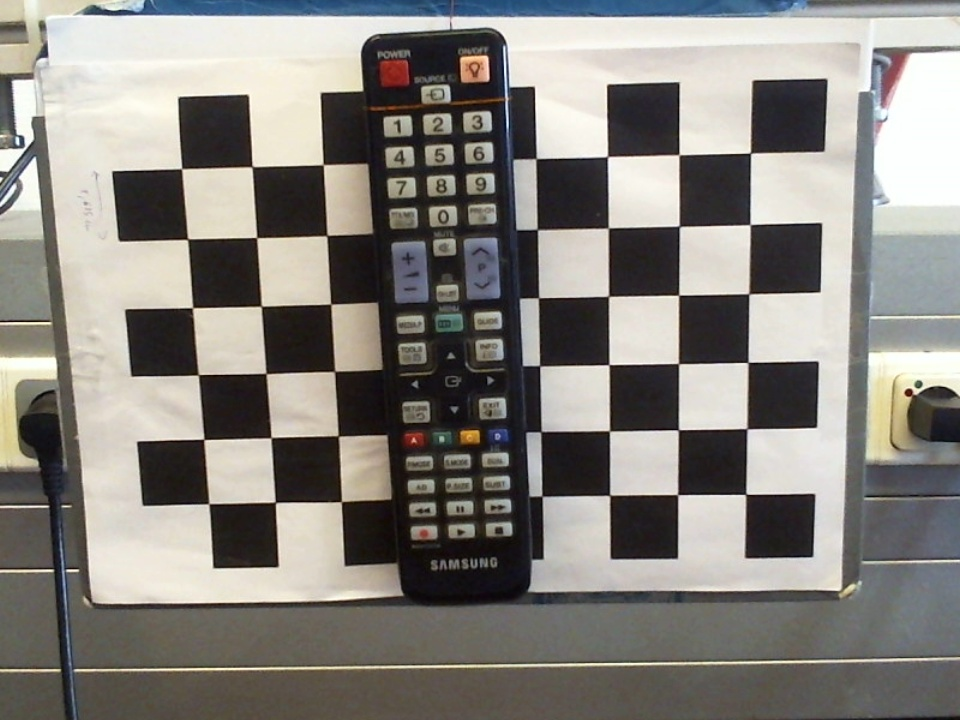
\includegraphics[width=\linewidth]{chapters/implementation/3dreconstr.jpg}
\caption{A rekonstrukcióhoz használt elrendezés. A rekonstruálandó tárgy egy TV-távirányító.}
\label{fig:reconstr-img}
\end{figure}

\subsection{A pozíció és orientáció meghatározásának implementációja}

A pozíció és orientáció meghatározása a PnP algoritmus RANSAC elvű megvalósításával történik. Amennyiben ismerjük a kamera pozícióját a tárgy koordináta-rendszerében, a \eqref{eq:trf-lanc1} egyenlet alapján kiszámolhatjuk a tárgy és a robot koordináta-rendszerek közti transzformációt, $\mathbf{T}_{OR}$-t. Ennek az ismeretében pedig a tárgyhoz képesti tetszőleges célkonfigurációba irányíthatjuk a robotkart.

A tárgy pozíciójának meghatározásához a szoftver öt különböző nézőpontból készít képeket. Mindegyikhez megpróbálja meghatározni a kamera külső paramétereit, és végül a mellett a konfiguráció mellett dönt, amelyet a legtöbb inlier alapján sikerül meghatározni. Ez után kiszámítja azt a konfigurációt, amelyben a kamera egyenesen ránéz a \ref{fig:cel-konf-cam} ábrán bekarikázott gombra, és majdnem érinti a távkapcsolót , ahogy az a \ref{fig:megfog-konf} ábrán látszik. Ez a megfogási konfiguráció. A program azonban (lehetséges ütközéseket elkerülendő) a megfogási konfigurációhoz képest egy eltolt célkonfigurációba irányítja a robotot. A célkonfiguráció a világ koordináta-rendszerben pozitív $z$ irányban (fölfele) 20 cm-rel van eltolva a megfogási konfigurációhoz képest. Ezt a \ref{fig:cel-konf} ábrán látjuk.

\begin{figure}[H]
\centering     %%% not \center
\subfigure[Megfogási konfiguráció]{\label{fig:megfog-konf}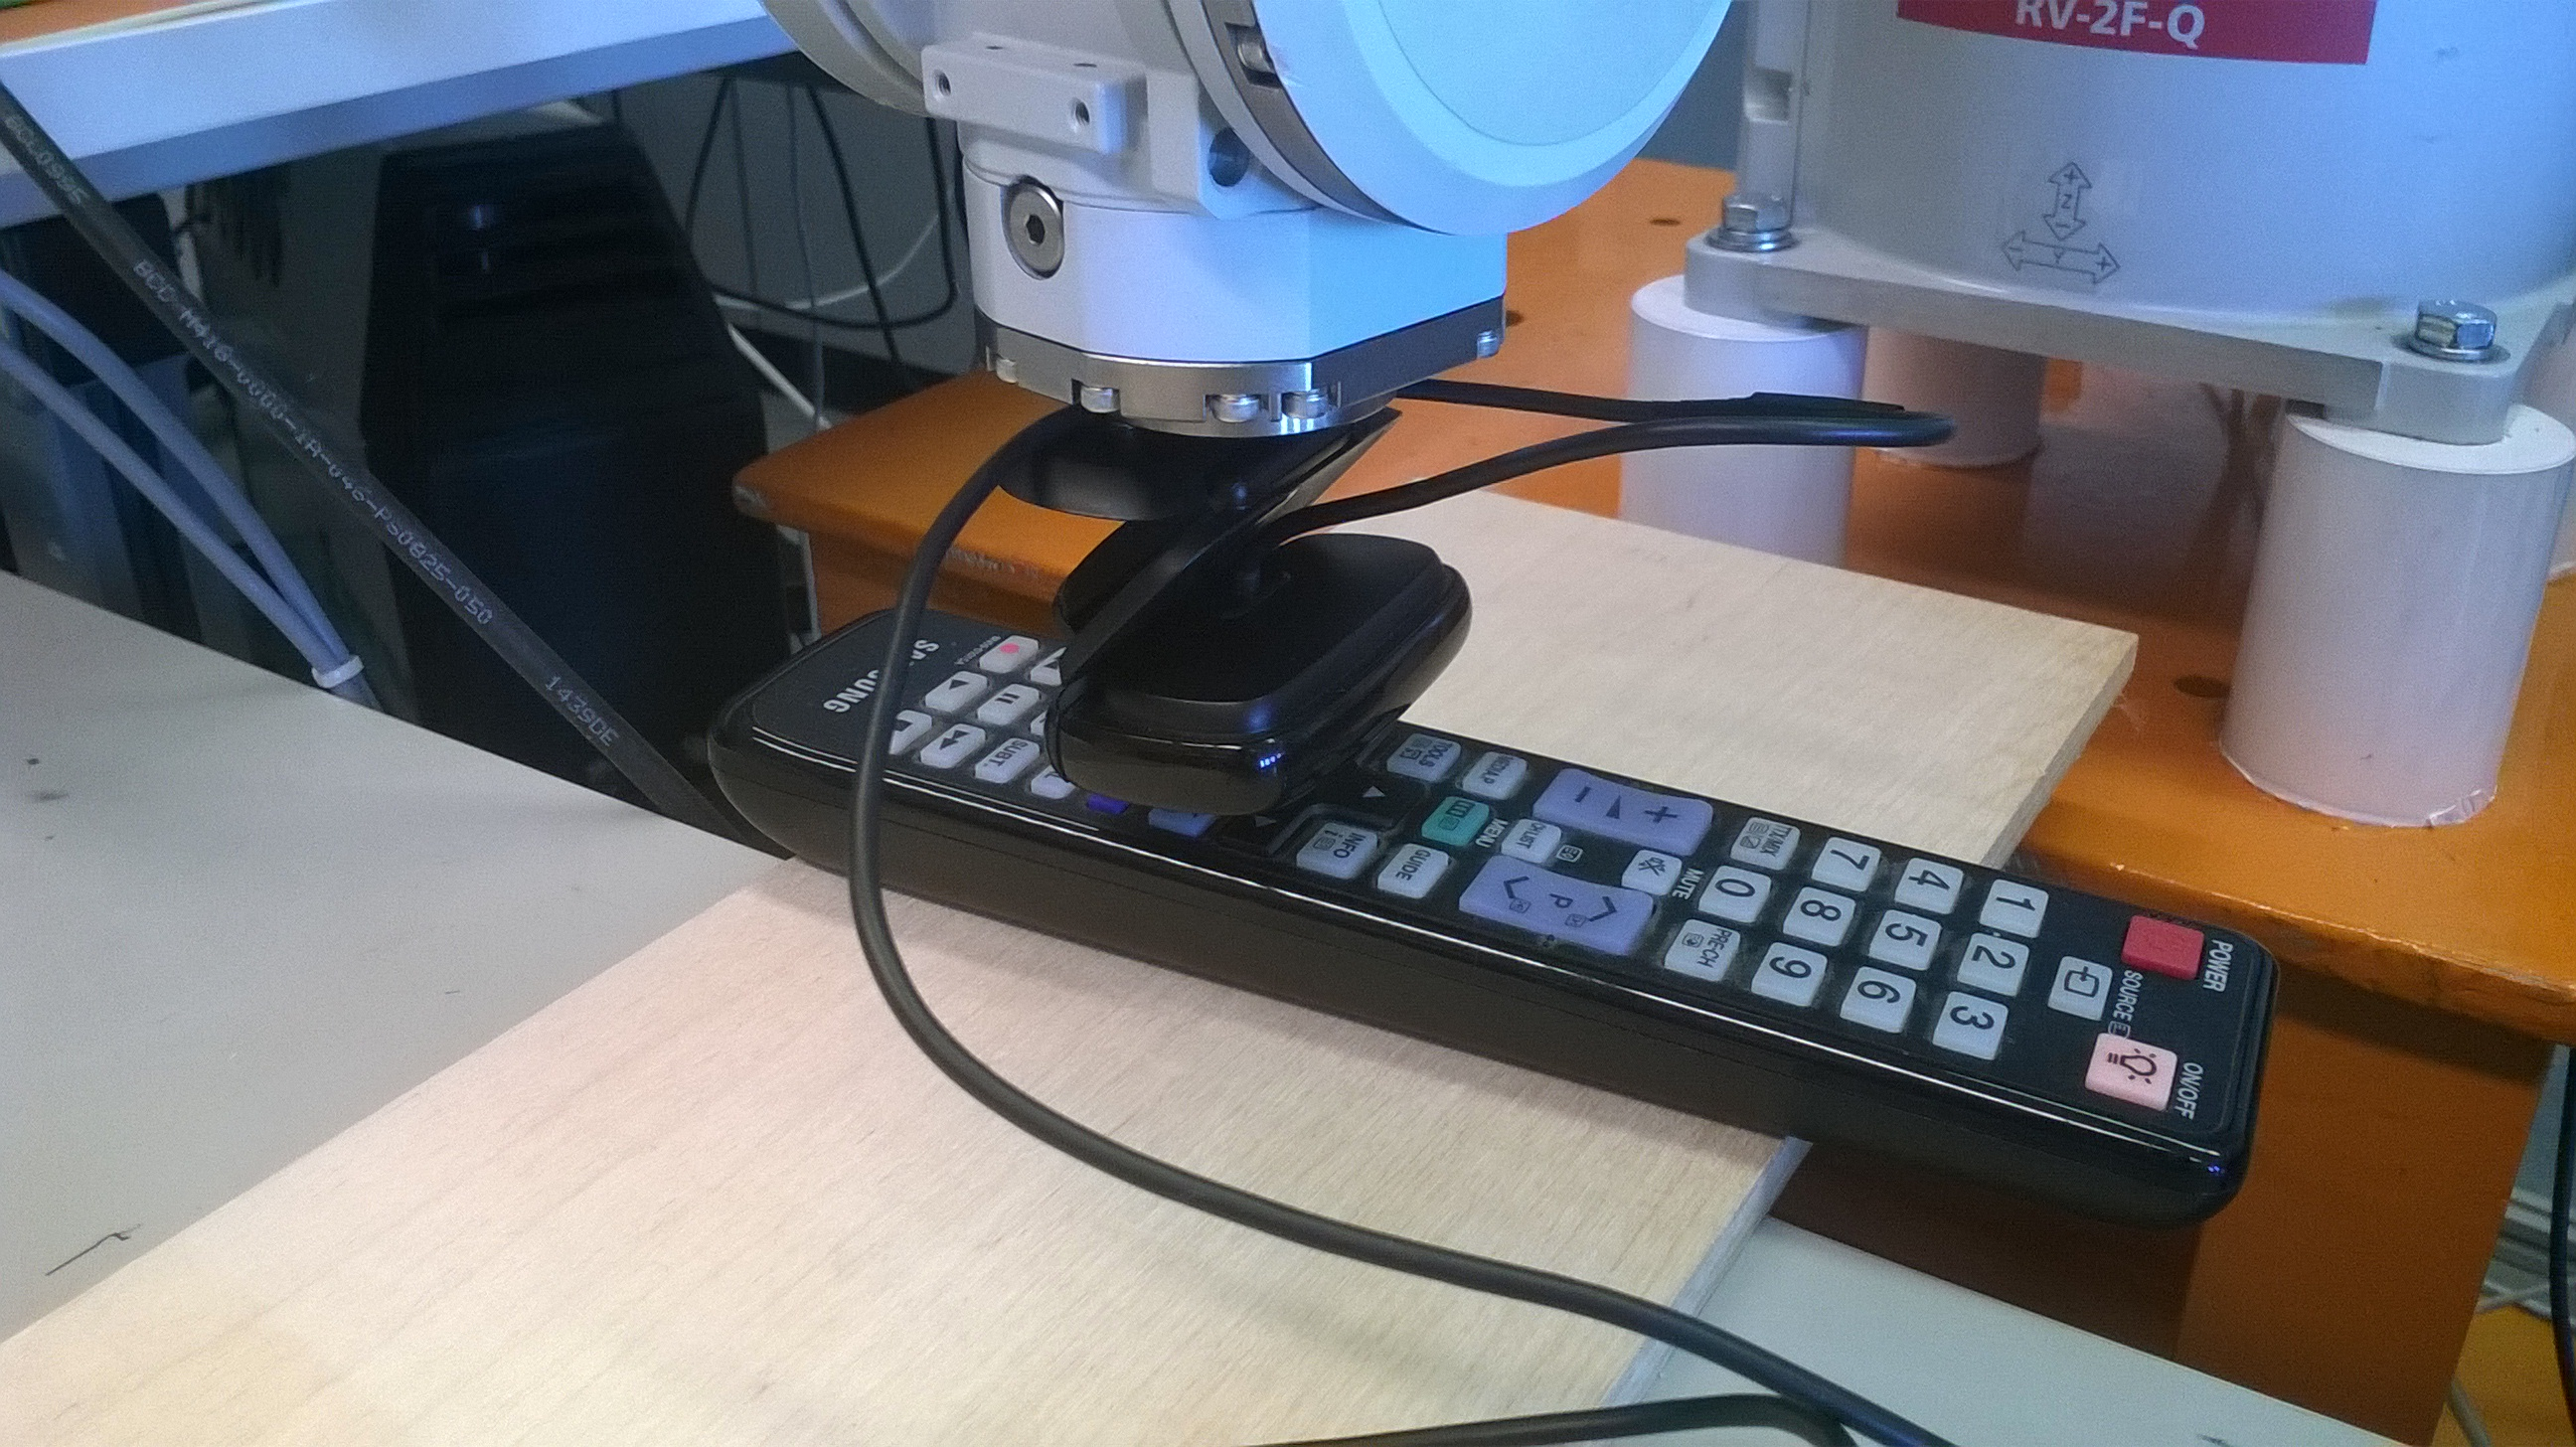
\includegraphics[width=0.45\linewidth]{chapters/implementation/megfog.jpg}}
\subfigure[Célkonfiguráció]{\label{fig:cel-konf}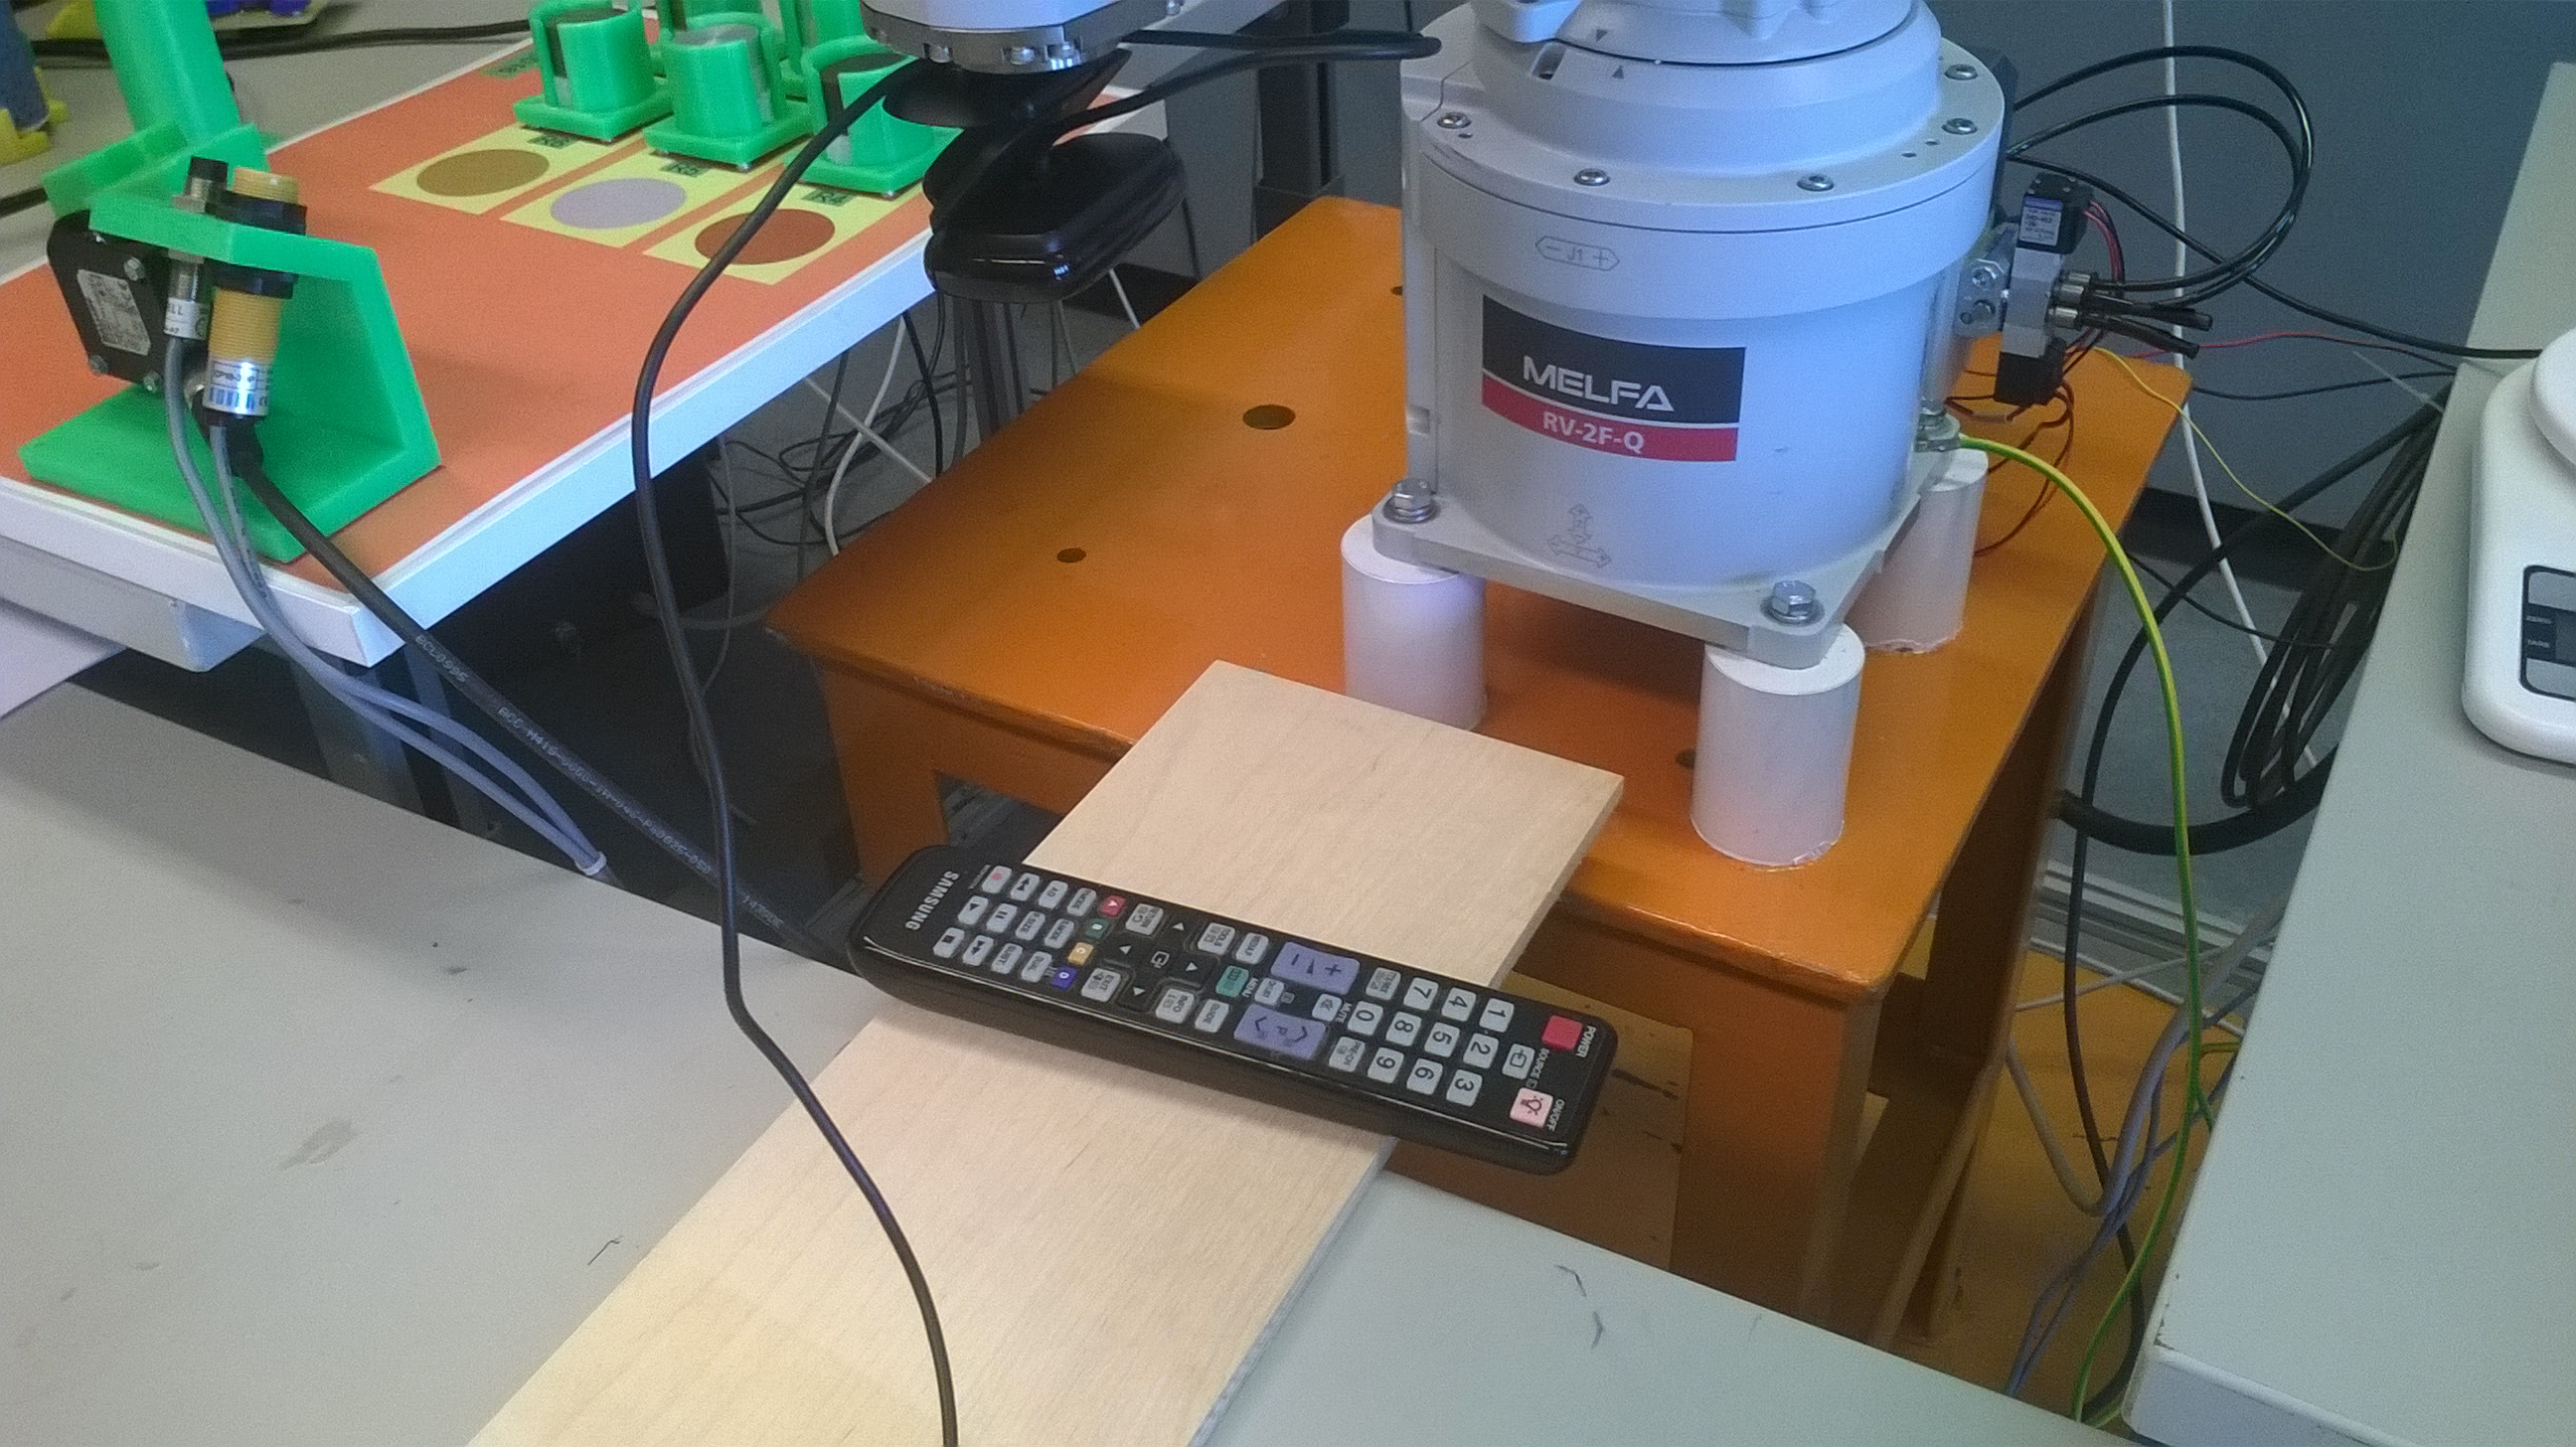
\includegraphics[width=0.45\linewidth]{chapters/implementation/cel.jpg}}
\subfigure[A kamera képe a célkonfigurációban.]{\label{fig:cel-konf-cam}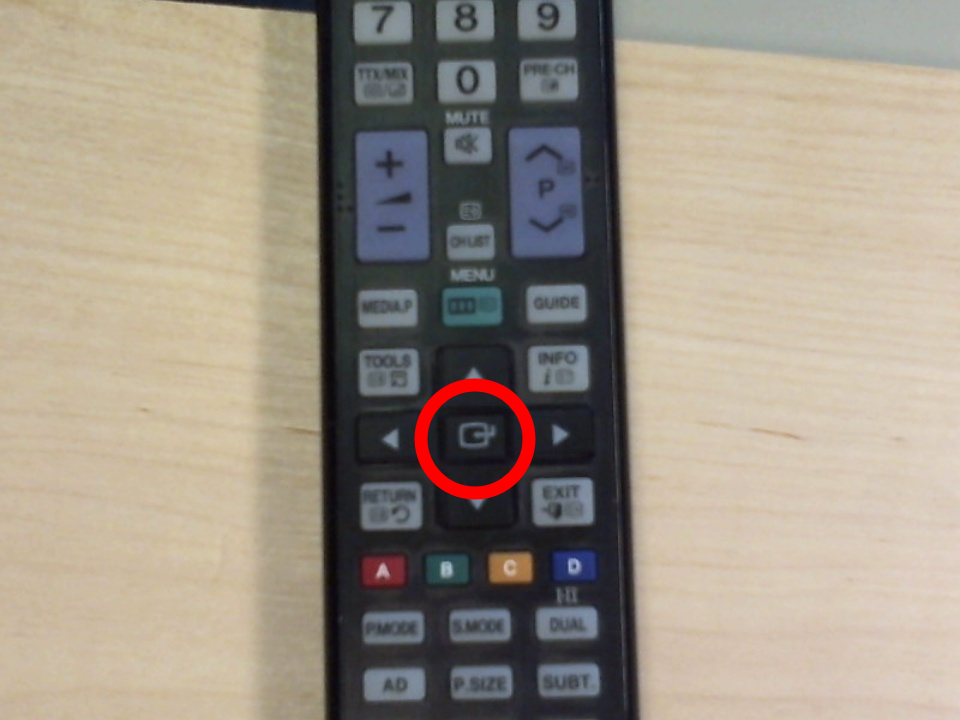
\includegraphics[width=0.45\linewidth]{chapters/implementation/cel_cam.png}}
\caption{A célkonfiguráció meghatározása}
\end{figure}

\section{A robotirányító rendszer felépítése}
	A komplett rendszer hardverkomponensei között lévő kommunikációs lánc a következő elemekből épül fel:
	
\begin{enumerate}
\item PC
\item PLC (Q03UDVCPU)
\item Robotvezérlő modul (Q172DRCPU)
\item Robotkar (Melfa RV-2F-Q)
\end{enumerate}	

	A kommunikáció a következő módon valósul meg. A PC és PLC között a kommunikáció Modbus/TCP kapcsolaton keresztül történik, a PLC a belső hálózaton DHCP-vel kiosztott statikus IP-n elérhető. A Modbus/TCP egy Ethernet-alapú kommunikációs protokoll, amelyben a szerver elérhetővé teszi a hozzá csatlakozott kliensek számára a regisztereit, azok szabadon írhatók, olvashatók. A PLC és a robotvezérlő modul megosztott memórián keresztül kommunikálnak. A robotvezérlő közvetlenül irányítja a robotkart, azzal egy komplett berendezést alkot, a köztük lévő kommunikáció megoldása nem a felhasználó feladata.
	
\begin{figure}[H]
\centering
\includegraphics[width=\linewidth]{chapters/implementation/system.png}
\caption{A robotirányító rendszer felépítése.}
\end{figure}
	
	A robot megfogójára egy Logitech c525 típusú webkamera van szerelve, ez szolgáltatja a képfeldolgozás számára a vizuális információt.
	
	
\begin{figure}[H]
\centering
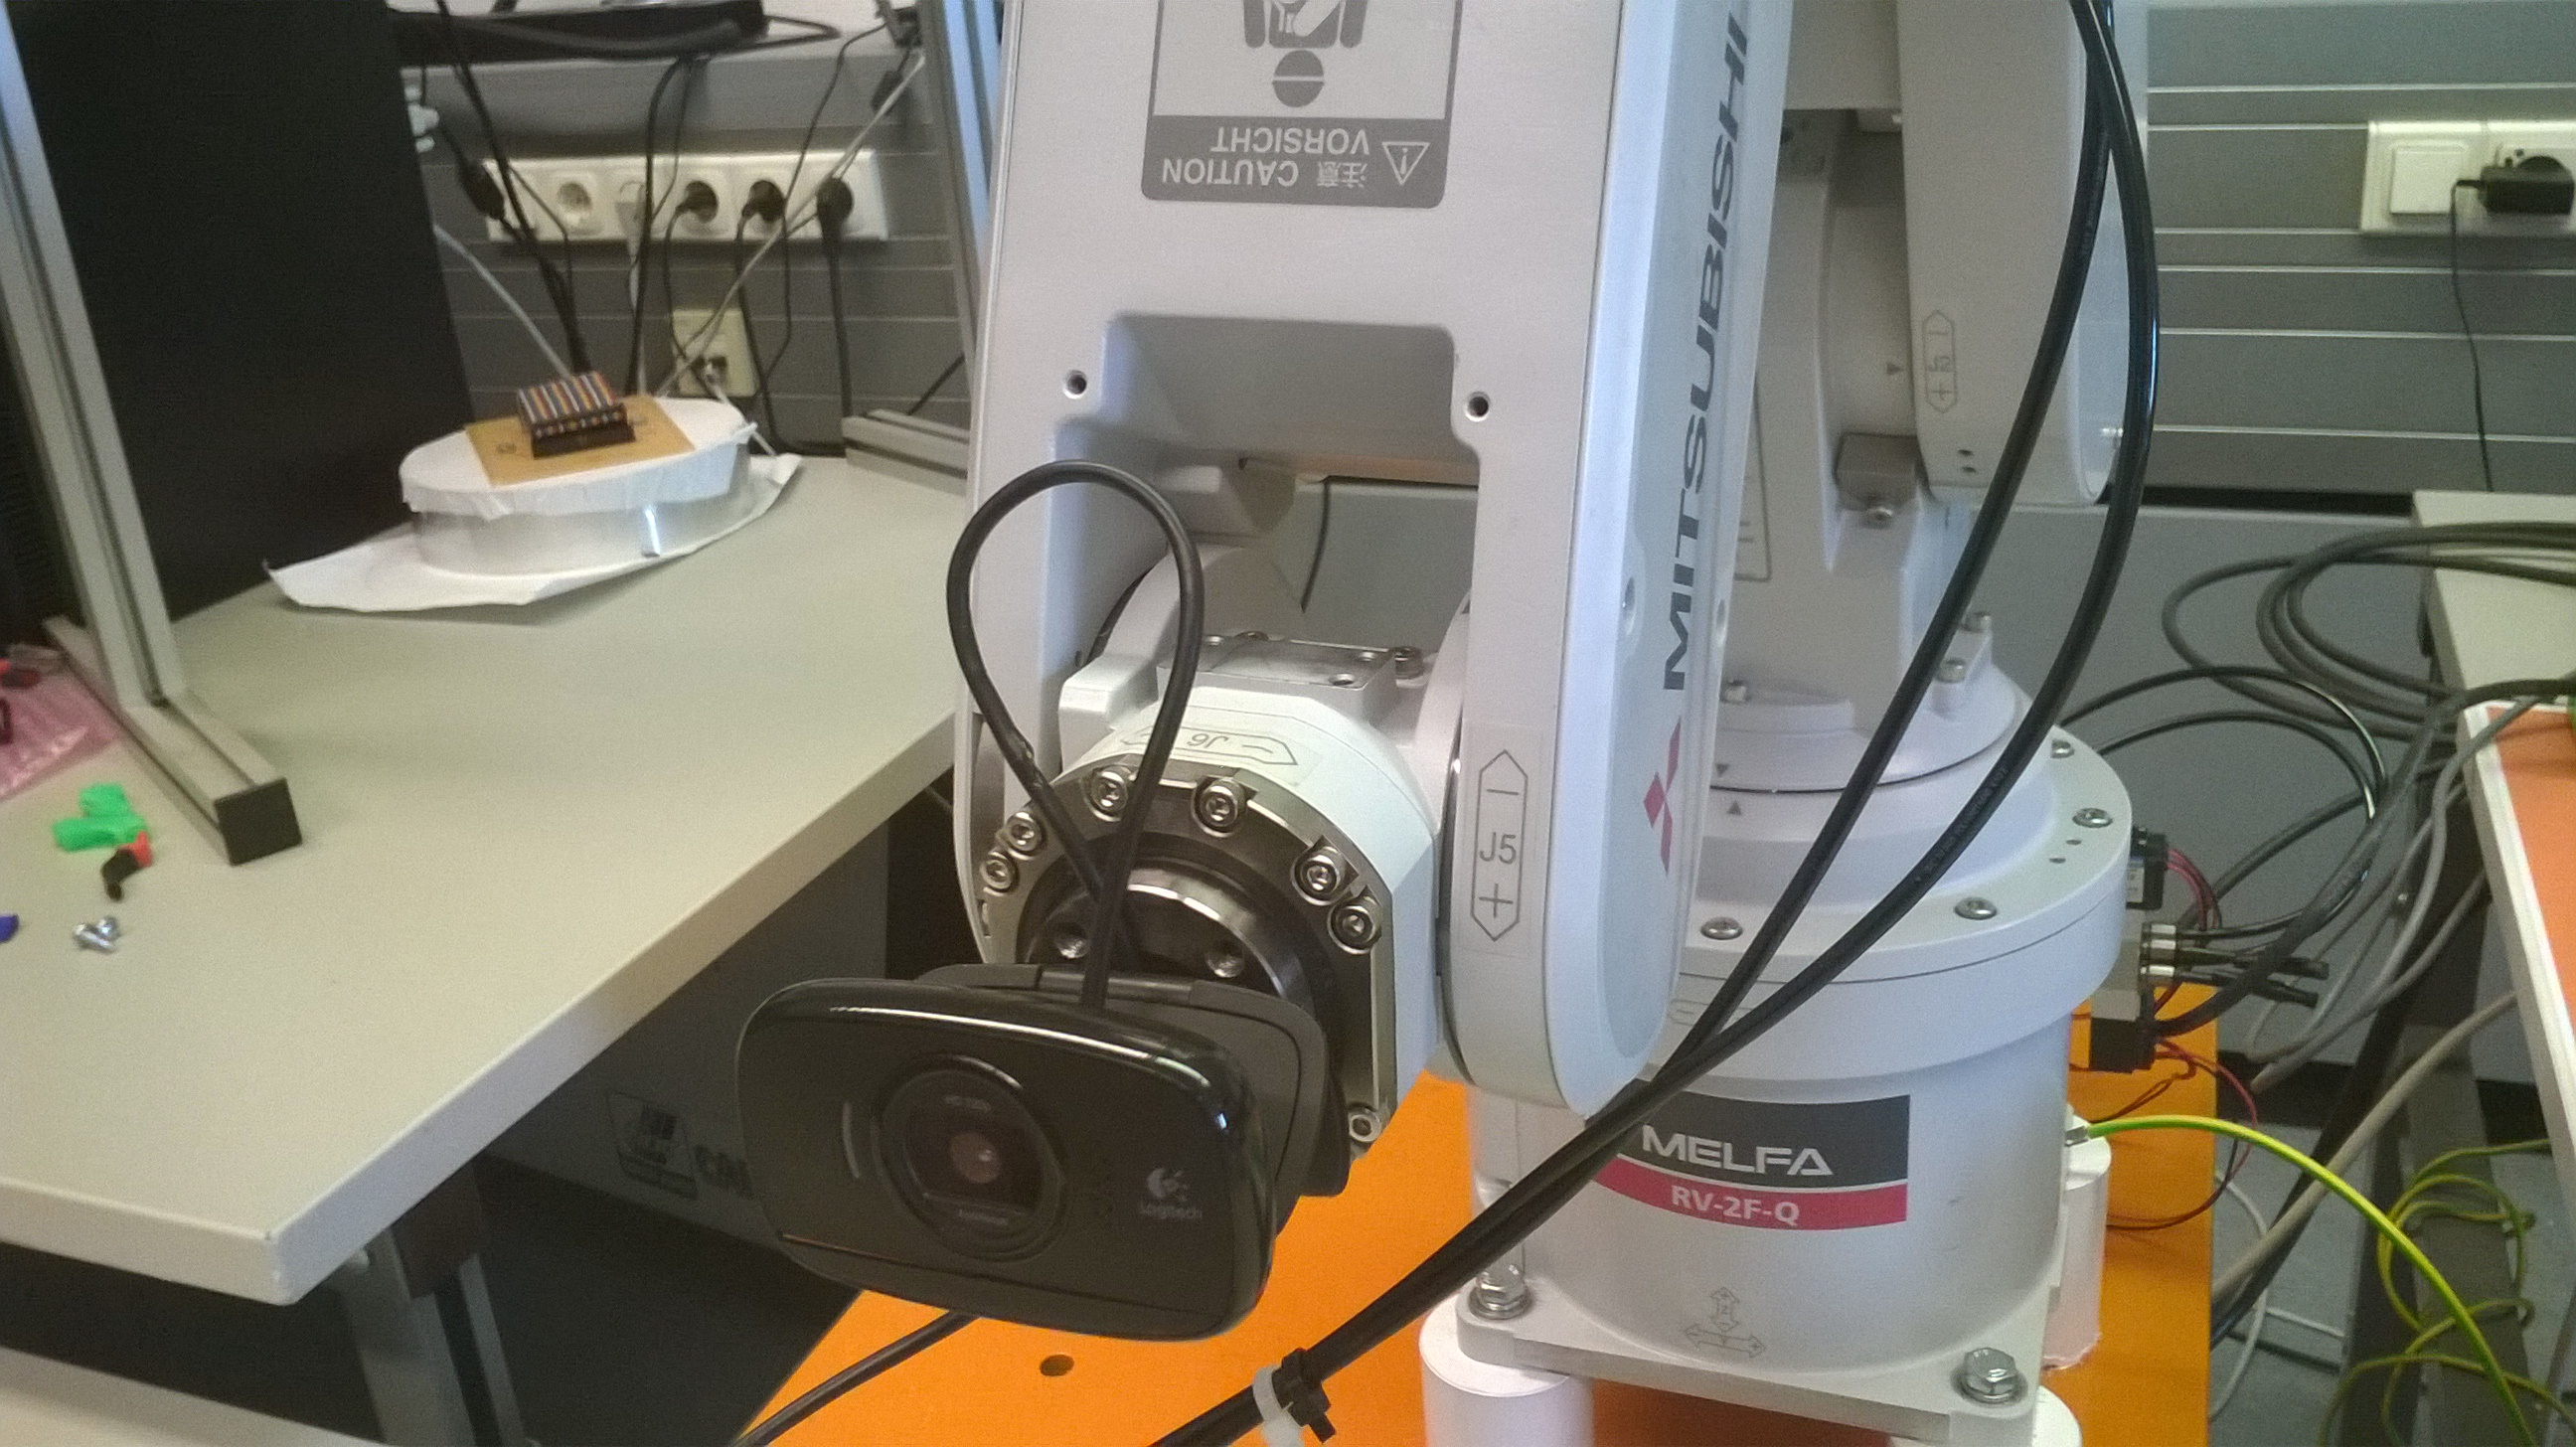
\includegraphics[width=\linewidth]{chapters/implementation/robocam.jpg}
\caption{A robotra szerelt kamera.}
\end{figure}
	
	\section{A PLC és robotprogram}
	
	A PLC-n két, a működéshez szükséges program fut. Az egyik egy Modbus szerver, ami a PC-vel való kommunikációt kezeli. Ez a Mitsubishi cég (és a programot korábban felfedező és használó hallgatók) jóvoltából már rendelkezésre állt számomra. 
	
	A másik program a robot felé történő kommunikációért felelős. Minthogy a PLC csak összekötő szerepet játszik a robot és a PC között, ezért ennek a programnak a feladatköre arra korlátozódik, hogy a Modbus-on keresztül kapott értékeket továbbítsa a megosztott memóriába. Ezt a programot Menyhárt Balázs MSc hallgató készítette, én minimális módosításokkal az ő programját használom.
	
	A roboton futó program kiolvassa a megosztott memóriából a megfelelő értékeket, és ennek megfelelően mozgatja a robotkart. Ennek a megvalósítása úgy történik, hogy egy-egy regiszterben kerül átadásra a pozíció-orientáció 6 paramétere. A robotprogram elvégzi a megfelelő korrekciókat (szög-radián átváltás), majd a megadott helyzetbe irányítja a megfogót. Ez ki van még egészítve egy utasításszámlálóval, amelynek értékét a PC-n futó programban vizsgálva megtudhatjuk, hogy az adott utasítást a robot elvégezte-e már.

	\section{A PC program}
	
	A PC programot Python nyelven írtam. Képfeldolgozásra az OpenCV függvénykönyvtárat, a Modbus kommunikáció megvalósításához a PyModbusTCP könyvtárat használtam.

	Csatlakozás után a megadott helyzetbe lehet irányítani a robotot, illetve a megfelelő gomb megnyomásával a kéz-szem kalibráció és a tárgy megkeresése is elvégezhető.
	
\begin{figure}[H]
\centering
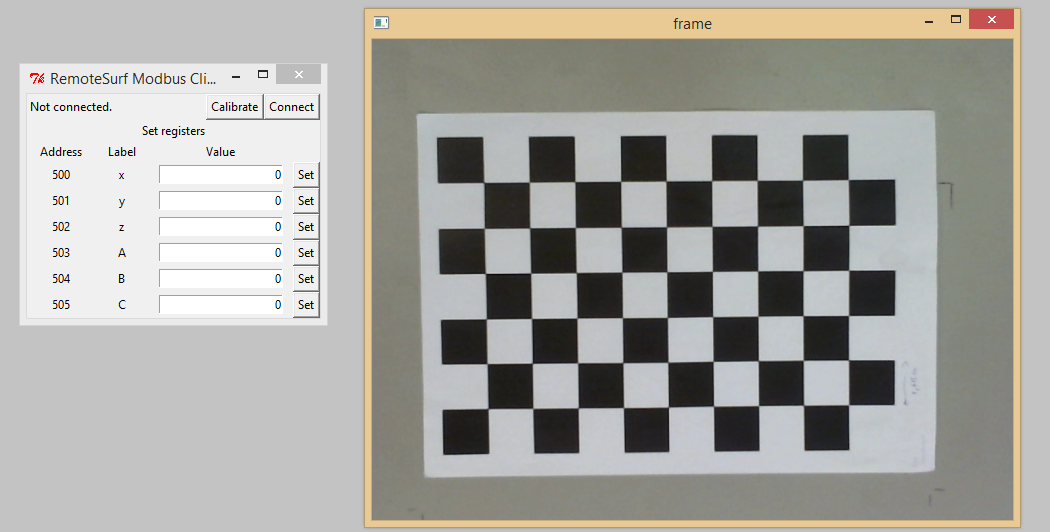
\includegraphics[width=\linewidth]{chapters/implementation/gui.png}
\caption{A program felhasználói felülete.}
\label{img-gui}
\end{figure}

	A legtöbb általam használt algoritmus OpenCV-s implementációját használom. Saját implementációk közül a legfontosabb a kéz-szem kalibráció algoritmusa és az \ref{muli-view-triang} fejezetben ismertetett háromszögelés algoritmusa. 
		
	A Kabsch algoritmust implementáló kódrészt Jimmy Charnley Kromann és Lars Andersen Bratholm írta, az ő kódjukat használom \cite{kabschGithub}.
	